\documentclass[12pt, a4paper]{article}
 
%Bibliography
%\usepackage[backend=biber,citestyle=numeric]{biblatex}
\usepackage{graphicx}
%\addbibresource{interim.bib}
 \usepackage{longtable}
%Customise layout of Contents page
\usepackage{tocloft}
%\usepackage{caption}
%\usepackage{subfigure}
\usepackage{float}
%Hyperlinks in contents
\usepackage[hidelinks]{hyperref}
%Dotted lines in table of contents
\renewcommand{\cftsecleader}{\cftdotfill{\cftdotsep}}
 
%Appendices
\usepackage[toc,page]{appendix}
 
\begin{document}
 
 
 
%%%%%%%%%%%%%%%%%%%%%%%%%
%       TITLE PAGE      %
%%%%%%%%%%%%%%%%%%%%%%%%%
 
        %Set alphabetic page numbering just for title page.
        \pagenumbering{alph}
       
        \begin{titlepage}
                       
                \center
               
                {\large Electronics \& Computer Science}\\
                {\large Faculty of Physical and Applied Sciences}\\
                {\large University of Southampton}\\[2.5cm]
               
                {\Large Tim Brooks}\\[0.5cm]
                {\Large \today}\\[2.5cm]
               
                {\LARGE Face Recognition in the Wild}\\[3.0cm]
               
                {\Large First Examiner: Dr Jonathan Hare}\\[0.5cm]
                {\Large Second Examiner: Dr Mark Nixon}\\[3.2cm]
                {\Large A Project Progress Report \\\ Submitted For The Award Of:}\\[0.2cm]
                {\Large BSc Computer Science}
               
                \vfill
       
        \end{titlepage}
       
        %Set page numbering back to numerical for rest.
        \pagenumbering{arabic}
       
       
       
%%%%%%%%%%%%%%%%%%%%%%%%%
%        ABSTRACT       %
%%%%%%%%%%%%%%%%%%%%%%%%%
 
        \begin{abstract}
               OpenIMAJ is an award winning set of libraries and tools for image manipulation. Currently, a pipeline for Face Recognition in the Wild has not been implemented in OpenIMAJ, this project is implementing a Face Recognition in the Wild pipeline, and investigating it’s effectiveness against other methods. \\
This report is to detail the progress made so far on the project of Face Recognition in the Wild. Four main areas of the project progress are examined. From these, conclusions have been drawn detailing how the project has progressed. So far, the Evaluation methods have been completed, ready for the development of the pipeline. It can be seen that the project has not reached the expected stage initially set out at the beginning, and considerations from this have been made to create an outline of remaining work to be completed. 
        \end{abstract}
       
        \newpage
       
 
%%%%%%%%%%%%%%
%  CONTENTS  %
%%%%%%%%%%%%%%
 
        %Display 'Page' header above the page numbers column.
        \addtocontents{toc}{~\hfill\textbf{Page}\par}
       
        %Make tabel of contents (Needs two typesetting runs to populate)
        \tableofcontents
       
 
%%%%%%%%%%%%%%%%%%%%%%%%%
%      MAIN CONTENT     %
%%%%%%%%%%%%%%%%%%%%%%%%%
 
        \newpage
 \section{Project Introduction and Goals}
 \subsection{Introduction}
 Faces are used by humans as a way of recognising individuals. Over the past few decades, algorithms have been developed that can recognise faces. These algorithms are constantly improving, as more and more technology is beginning to use Face Recognition. Face Recognition in the wild is the process of detecting and recognising faces that are not fully aligned to the camera, from more natural pictures. Face Recognition is a more trivial use of Face Detection, it incorporates recognition into detecting and recognising who the face belongs to. Currently, a Face Recognition pipeline has been implemented in OpenIMAJ, but it has not been very well tested, nor does it make use of the most effective method for Face Recognition.

 \subsection{Goals}
The aim for this project is to investigate and implement the method of Face Recognition used in \cite{simonyan2004fisher} in OpenIMAJ. This method is a pipeline of many state of the art features in Face Recognition, some already used in OpenIMAJ. This project will investigate those and use them in the final implementation. When the method has been implemented into OpenIMAJ, the project will explore the performance of the method against the expected results, and the results against other methods, including the state of the art High Dimensionality Local Binary Patterns (High-LBP) \cite{highlbpsift}, and others, time permitting. An aim of the project is to design it such that it is similar to the design ideology of OpenIMAJ, having very high cohesion between objects.

\newpage
\section{Background and report of literature search}
\subsection{History of Face Recognition}

\subsection{Face Recognition Techniques}
Face Recognition is the process of verifying or identifying the person in the image inputted. Depending on the type of application, there are many different methods that may be suitable to use. \cite{facesurvey} describes Feature-based and Hollistic approach to face recognition. Feature based works by analysing the image and identifying any features that would be of interest (such as the eyes). They are then extracted, and a dataset is built by calculating the geometric relationship between each point (for example the distance between the eyes and mouth). The data is then analysed to match the faces to the measurements. A Hollistic approach to face recognition involves the identification of faces by basing the descriptions on the entire face, as opposed to local features of the faces. This can be carried out either statistically, or using AI. By using statistical approach, an array of pixel intensity values are created, and direct comparison between each face is carried out. The AI method uses tools such as neural networks and machine learning to learn and recognise the faces.
\subsubsection{Eigenfaces}
Eigenfaces is the method of representing an image as a set of eigenvectors. First used for face classification by Turk and Pentland [reference paper],  they show that Eigenfaces are a practical solution to the problem of face recognition. Eigenfaces works by creating low dimensional feature vectors by applying Principal Component Analysis to feature vectors of the image. A classifier can then be trained to test and use the system. Turk and Pentland originally used KNN Classification, however any classification can be used. They 
\subsubsection{Facebook Deepface}


\subsection{Fisher Vector Faces in the Wild}
The paper Fisher Vector faces in the Wild \cite{simonyan2004fisher} shows that when Fisher vectors are used alongside densely sampled SIFT features, the resulting feature based face recognition system is capable of achieving state-of-the-art face verification performance on the Labelled Faces in the Wild \cite{labelledFaces} dataset. The paper proceeds to discover how a compact descriptor can be learnt from the fisher vectors using discriminative metric learning, since fisher vectors are highly dimensional. The conclusion of this paper is supported by a set of tables and graphs, detailing the results of tests on the Labelled faces in the wild dataset. Two methods are used to test the algorithm, the unrestricted setting where outside training data is used, and the restricted setting where no outside training data is used. It shows that when tested under the unrestricted setting, the pipeline has the second highest mean classification accuracy at 0.9303 with a slightly smaller error margin. This is second to High-Dimensionality LBP at 0.9318. In a restricted setting, the method yielded the highest accuracy of 0.8747, meaning it is the new state-of-the-art setting. The paper describes the steps it took in order to achieve it’s results, which uses many advanced facial recognition methods. In this literature review, the methods used will be examined, along with work related to Face Recognition.

In \cite{simonyan2004fisher}, there is a description of the processing pipeline used to achieve the high standard of facial recognition. This consists of the following parts:
\begin{itemize}
\item Facial landmark detection
\item Align and crop face
\item Dense Scale Invariant Feature Transformation, Gaussian Mixture Modelling and Fisher Vector Encoding
\item Discriminative Dimensionality Reduction
\item Compact Face Representation
\end{itemize}


\subsection{Dense SIFT}


\subsection{Fisher Vector Encoding}
Fisher Vectors describe a set of local features in a single vector. Fisher Vector encoding is the process of combining a large set of vectors into a high dimensional vector representation. By applying a Gaussian Mixture Model (GMM) on the vector elements, the derivatives of the log-likelihood of the model can be encoded with respect to it’s parameters. By using the set of local features from Dense SIFT, a highly dimensional Fisher vector can be created. The GMM is seen as a face model, and if plotted on the image, the mean and variance of GMM’s are represented by ellipses of all the features. A representation can be created between the features and the GMM centres by training a GMM with diagonal covariances, then calculate the derivatives with respect to the Gaussian mean and variances. A more detailed explanation is available in \cite{simonyan2004fisher}, showing the functions used to create the vectors.

\subsection{Large-Margin Dimensionality Reduction}

Large-Margin Dimensionality Reduction is the step in which the Fisher Vectors are compressed to small discriminative representation. This stage is where the calculation is made that determines if the two given faces are the same or not. \cite{simonyan2004fisher} details the method, explaining how a high dimensional fisher vector can be projected to a low dimensional vector, in order for the squared euclidian distance can be calculated. If the squared euclidian distance between the two images are smaller than a threshold, then they are the same person in the image.
        
  \subsection{Labelled Faces in the Wild Dataset}

The Labelled Faces in the Wild Dataset is a database of images collected for the purpose of testing face recognition systems. The main problem it is used for is such that, “Given two pictures, each of which contains a face, decide whether the two people pictured represent the same individual” \cite{labelledFaces}. The database contains 13,233 images, of 5,749 different individuals. 1680 individuals have two or more images in the database, whilst 4,069 have just one. The database contains a wide variety of faces, varying on many factors including pose, lighting, expression, background, race, ethnicity, age, gender, clothing, hairstyles, camera quality, colour saturation and focus. This give a wide range of samples to use in order to test the face recognition system.

The way that this dataset works is by using the pre-defined views (sets of images, some positively matching and others negatively matching). The first is for algorithm development, and the second is for performance reporting. Using these two different views helps ensure that the algorithm will not be skewed for the final results.

For example, given the following two images of Jon Stewart (Figure 1) and  Paul McCartney (Figure 2), the algorithm should correctly classify these as not being the same person. 

\subsection{OpenIMAJ}
OpenIMAJ is an Open Intelligent Multimedia Analysis toolkit for Java \cite{openimaj}. It consists of a set of libraries and tools used for multimedia content analysis and content generation. OpenIMAJ already utilises several components needed for the Fisher Vector face recognition implementation. It contains the necessary code for Facial Landmark Detection, Align and Crop,  Dense SIFT, Principal Component Analysis. 
For Facial Landmark Detection, there is a class in OpenIMAJ that can be used, the FKEFaceDetector (Front Keypoint Enriched Face Detector). There is also the AffineAligner that can be used in order to perform the Align and Crop face. 


\begin{figure}[H]
\minipage{0.45\textwidth}
  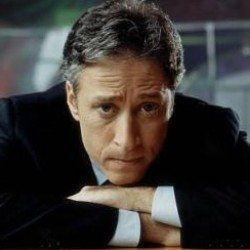
\includegraphics[width=\linewidth]{images/Jon_Stewart_0001.jpg}
  \caption{Jon Stewart}
\endminipage\hfill
\minipage{0.45\textwidth}
  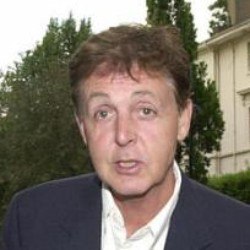
\includegraphics[width=\linewidth]{images/Paul_McCartney_0004.jpg}
  \caption{Paul McCartney}
\endminipage\hfill
\end{figure}
Whereas, given these two images of Mark Wahlberg (Figure 3 and Figure 4), the algorithm should correctly classify these as being the same person.

\begin{figure}[H]
\minipage{0.45\textwidth}
  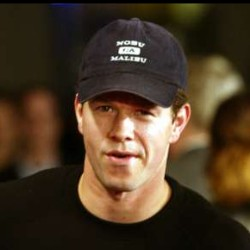
\includegraphics[width=\linewidth]{images/Mark_Wahlberg_0001.jpg}
  \caption{Mark Wahlberg}
\endminipage\hfill
\minipage{0.45\textwidth}
  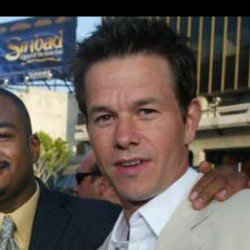
\includegraphics[width=\linewidth]{images/Mark_Wahlberg_0004.jpg}
  \caption{Mark Wahlberg}
\endminipage\hfill
\end{figure}

\newpage
%\section{Analysis}
\section{Analysis}
\subsection{Requirements}
A requirements specification has been created for an implementation of an algorithm, using research discussed in section 2. Functional Requirements describe what the project will do. Non-functional requirements explain how the project will do so. \\

\textbf{Functional Requirements}
\begin{itemize}
\item The project will use the Fisher Vector encoding face recognition pipeline used in \cite{simonyan2004fisher}.
\item The project will compare two images and output if they are the same or not. The ability to assess if two images are the same is a basic requirement of face recognition.
\item The project will use the Labelled Faces in the Wild image dataset - The Labelled Faces in the Wild dataset is a very common dataset used to test the effectiveness of face recognition algorithms. By using this dataset, I am able to compare to published results of other face recognition methods - including the results achieved by \cite{simonyan2004fisher}.
\item The project will be able to evaluate the results by creating a Receiving Operating Characteristic (ROC) curve. An ROC graph is created by plotting the proportion of true positives out of the total actual positives, against the fraction of false positives out of the actual total negatives, this is useful as it will allow comparison between the implementation and other face recognition methods.
\item The project will be able to evaluate by outputting a mean classification accuracy - the percentage of image pairs correctly classified. This will also help evaluate the implementation against the other face recognition methods.
\end{itemize}

\textbf{Non-functional}
\begin{itemize}
\item The project will be written in Java and be able to work with OpenIMAJ - The main aim of this project is to implement the face recognition in OpenIMAJ, a Java library.
\item Use existing classes in OpenIMAJ where possible. OpenIMAJ has many classes ready to be used, the implementation of this project will be in such a way that if there is an already existing method, it will be tested to ensure it’s effectiveness, and used.
\item Create each step of the pipeline individually, so they can be used standalone in the future. Such to the nature of OpenIMAJ, by ensuring that each algorithm used is implemented in it’s own class, it will be able to be used in other OpenIMAJ projects, not just this one. 
\end{itemize}
\subsection{Risks}
The table in Appendix A.1 Table 1 outlines the possible problems that would affect the project. Each problem has a an explanation, along with how much it would impact the project (in terms of the amount of time needed to overcome the problem). Along with that, a risk factor is given, determining how much of a risk the problem would be. As you can see, the highest risk is a hardware failure on the development machine, or data corruption. For each risk, a contingency plan has been created, detailing what would happen in each eventuality. A contingency plan has been created, as shown in Appendix A.2 Table 2. A contingency plan is very useful, as it will not only help overcome any problems in the project if they happen, but will help prevent those problems in the first place. 

\section{Design \& Implementation}
\subsection{Final Design}
This project has been split down into several sections in order to help structure the implementation of it. Each section is as follows:
\begin{itemize}
\item Evaluation Methods
\item Facial Landmark Detection
\item Dense SIFT
\item Gaussian Mixture Model
\item Fisher Vector Encoding
\item Discriminative Dimensionality Reduction
\item Compact Face Representation
\item Pipeline implementation
\end{itemize}
The way that the implementations have been planned allow a clear design structure to be concluded. Each implementation will be created as an individual class or set of classes. This will result in a highly cohesive project, helping with project management. In the long term it will encourage the reuse of code in other OpenIMAJ projects. The evaluation methods have been created first in order to allow for testing to take place throughout the project. Appendix B.1 shows a class diagram, showing outlines for the design of the pipeline, using pre-existing classes (e.g. AffineAligner), and new classes that will be created (e.g. FVEncode).

The project will run from command line to output the results for the evaluation. If time allows, this project may create a Graphical User Interface to run the evaluation tools, however, this is not a requirement for project success.
\subsection{Tools} 
This project will be developed using Eclipse as a development environment. Eclipse allows for easy cross platform integration, allowing the opportunity to work on Mac, Linux and Windows with ease. Eclipse has an advanced set of debugging tools available to be used, which will be of great help if the project comes in to any difficulties.\\ 
Whilst OpenIMAJ is going to be adapted in this project, it is also going to be used in development. OpenIMAJ contains several tools needed for implementing the face recognition method, and they will be tested to ensure suitability and used accordingly. \\
\LaTeX{} will be used to create and present the Project Brief, Progress Report and the Final Report. \LaTeX{} is a document preparation and typesetting program to output a report. This will give the project more flexibilty over the content of the reports, and allows the author present a professional report each time. To write the \LaTeX{}, the program TexMaker will be used. This program is a productive way to write \LaTeX{}, with a built in compiler, it outputs the document in the same window, allowing for fast writing and formatting.\\
BibTeX will be used to handle references in the \LaTeX{} document. This allows for fast and easy referencing in the reports. A separate .bib file is created in a text editor and populated with the references in the BibTeX format. They can then be easily used in the \LaTeX{} document.\\
To ensure that no work is lost, Git version control will be used in conjunction with a remote repository hosted privately on Github. Git is useful for several reasons. It is a way of backing up to a remote location, and so will reduce the effects of a large loss of work from a local workstation, as it will be available to access from Github. Being able to use version control is great for development, as new branches allow work to be carried out without affecting a master copy. This will be especially useful in the stages of the project where the face recognition method is being optimised to achieve the best results possible. Git will also be used to store and version control the Project Reports.

\section{Testing}
\subsection{Strategy}
\subsection{Results}

\section{Conclusions}

\section{Further Work}

%%%%%%%%%%%%%%%%%%%%%%%%%
%       APPENDICES      %
%%%%%%%%%%%%%%%%%%%%%%%%%
 
        \newpage
 
        \begin{appendices}
        
\section{Appendix A}
\subsection{Risk Table}
 \begin{longtable} {| p{1.7cm} | p{3cm} | p{6cm} | p{1.7cm} | p{2cm} |}  
\multicolumn{5}{c}
{\tablename\ \thetable\ -- \textit{Risks}} \\
    \hline
    \textbf{Risk ID} & \textbf{Risk} & \textbf{Outcome(s)} & \textbf{Impact} & \textbf{Risk Factor} \\ \hline
1 & Hardware failure on the main development machine & System would need rebuilding or hardware would need replacing. Would cause large delays & 5 & High \\ \hline
2 & Data corruption & Work would have to be restarted from the most recent backup. Depending on when the most recent backup was, this would cause large delays. & 5 & High \\ \hline 
3 & Authors personal issues (e.g. illness) & Could cause long term delays to the project development & 4 & High\\ \hline
4 & Misjudging time needed for the project & The whole project wouldn't be completed to it's full potential, this would affect the final outcomes as set out in the requirements & 3 & Medium\\ \hline
5 & Dataset no longer available & This would cause a number of issues and slight delays due to the evaluation method being based around the Labelled Faces in the Wild dataset. & 3 & Medium \\ \hline 
    \end{longtable}
    \newpage
\subsection{Contingency Plan Table}
 \begin{longtable} {| p{1.7cm} | p{12cm}| }  
\multicolumn{2}{c}
{\tablename\ \thetable\ -- \textit{Contingency Plan Table}} \\
    \hline
    \textbf{Risk ID} & \textbf{Contingency Plan} \\ \hline 
1 & In the event of a hardware failure on the main development machine, the contingency plan would depend on the project's progress. If this happened a few days before a major deadline, a new machine would be used to continue the work, provided there is a very recent backup. If it happened further from the deadline, or no backups have been made of the recent work, attempts to fix the machine would take place. \\ \hline
2 & In the event of data corruption, the most recent copy will be downloaded from the version control repository. A main reason why Git is being used at an external repository is for the backup functionality, hopefully preventing any data loss. This is only a successful plan if the author is consistent at using Git\\ \hline 
3 & In the event of the author having personal issues, advice would be sought after from the project supervisor and personal tutor, Dr. Paul Lewis and Dr. Enrico Costanza, and if necessary, further action will be taken to make the Faculty aware of the issues.  \\ \hline
4 & In the event of there not being enough time to complete the project due to poor time allocation, efforts would be focussed on completing as much as possible to achieve the minimum set out in the requirements. \\ \hline
5 & The dataset has been downloaded, so in the event of the dataset no longer being online to download, the project will not be affected. \\ \hline 
    \end{longtable}

\section{Appendix B}
\subsection{Class Diagram}
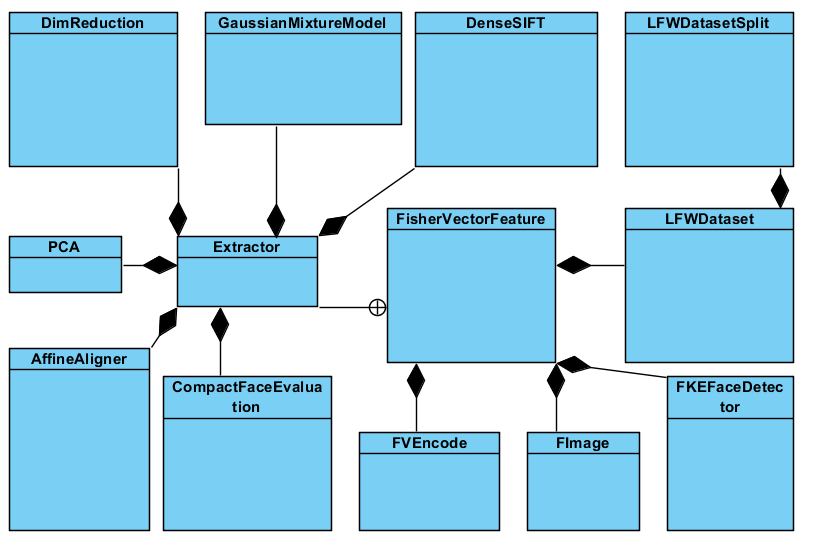
\includegraphics[scale=0.6, angle=0]{images/class.png}

\section{Appendix C}
\subsection{Preliminary Gantt Chart, work before Christmas}
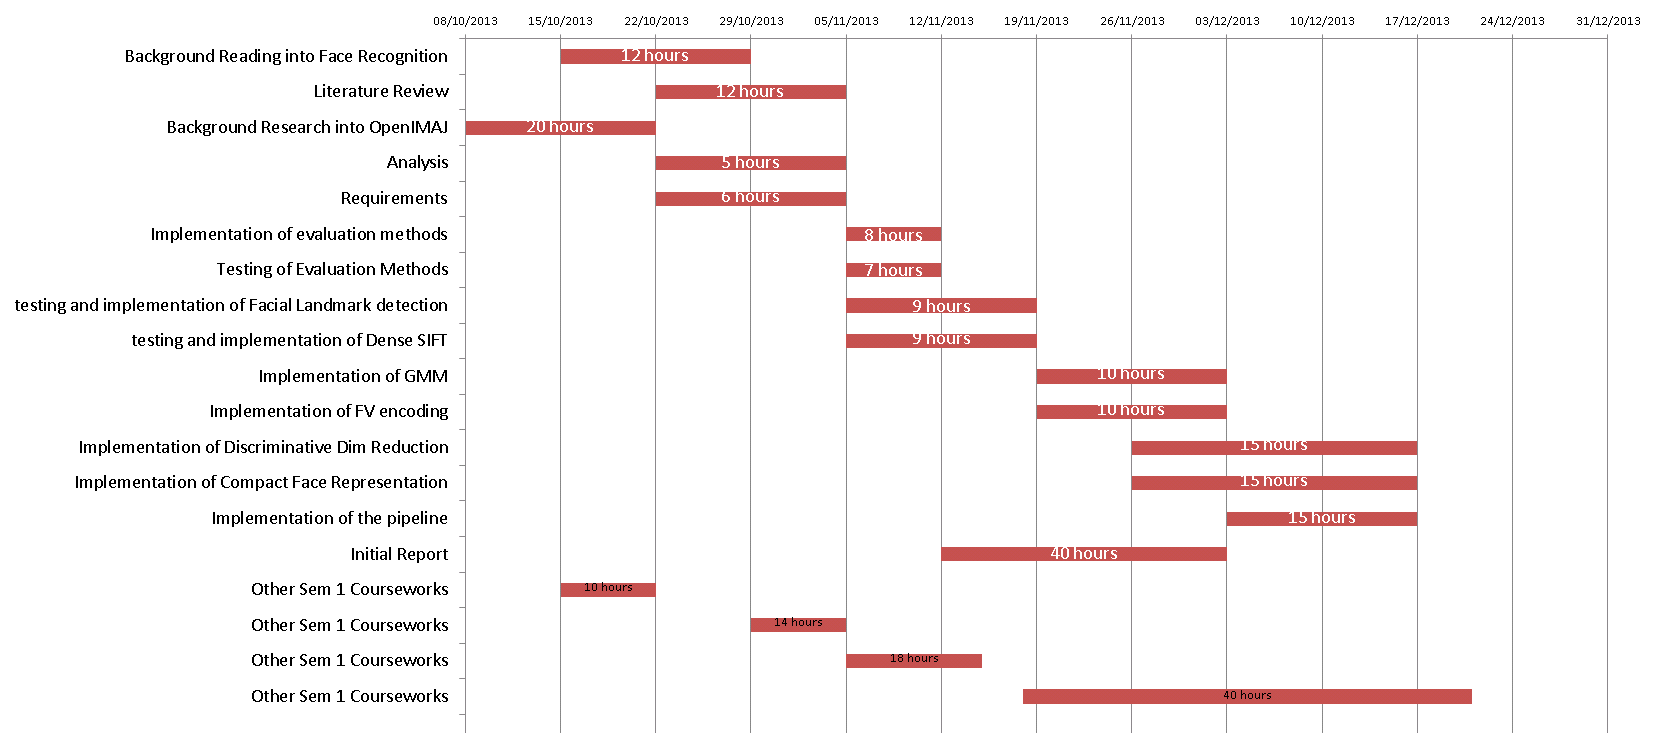
\includegraphics[scale=0.4, angle=90]{images/ganntFIRSTprexmas.png}
\subsection{Preliminary Gantt Chart, work after Christmas}
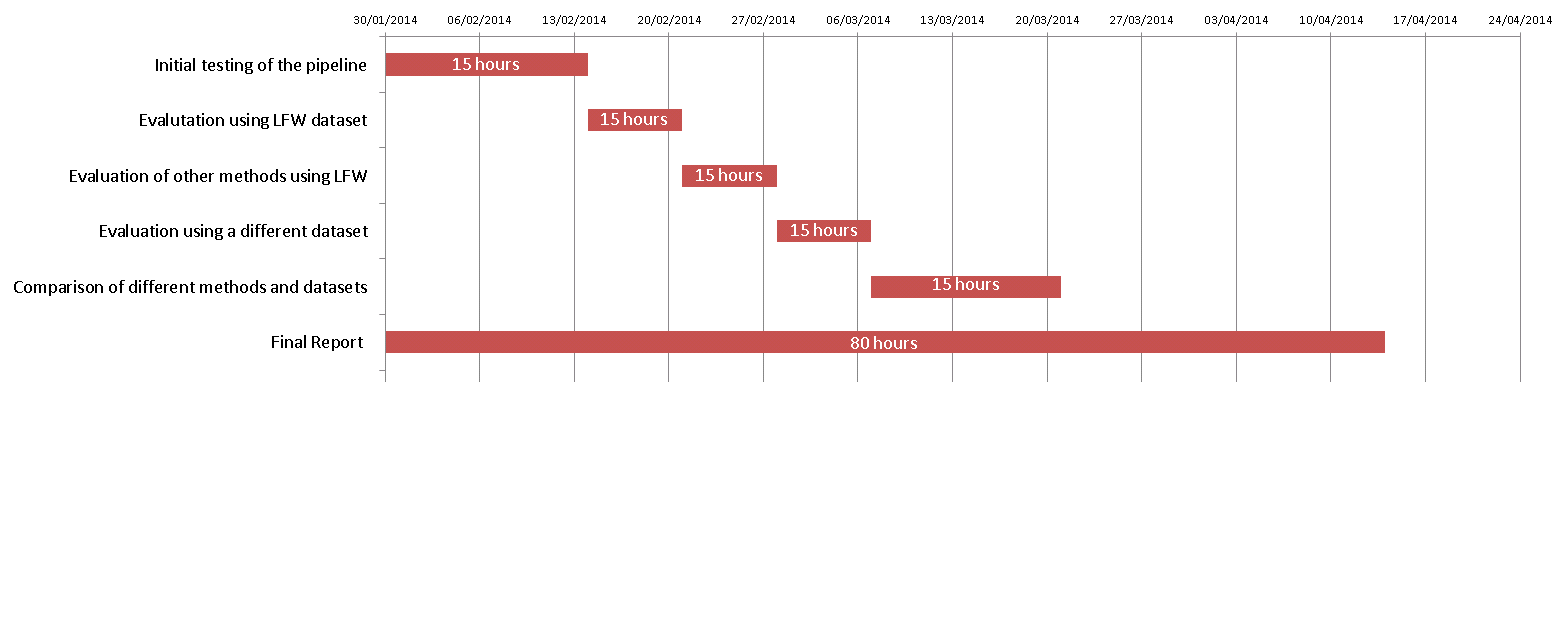
\includegraphics[scale=0.4, angle=90]{images/ganntFIRSTpostxmas.png}

\section{Appendix D}
\subsection{Updated Gantt Chart, work before Christmas}
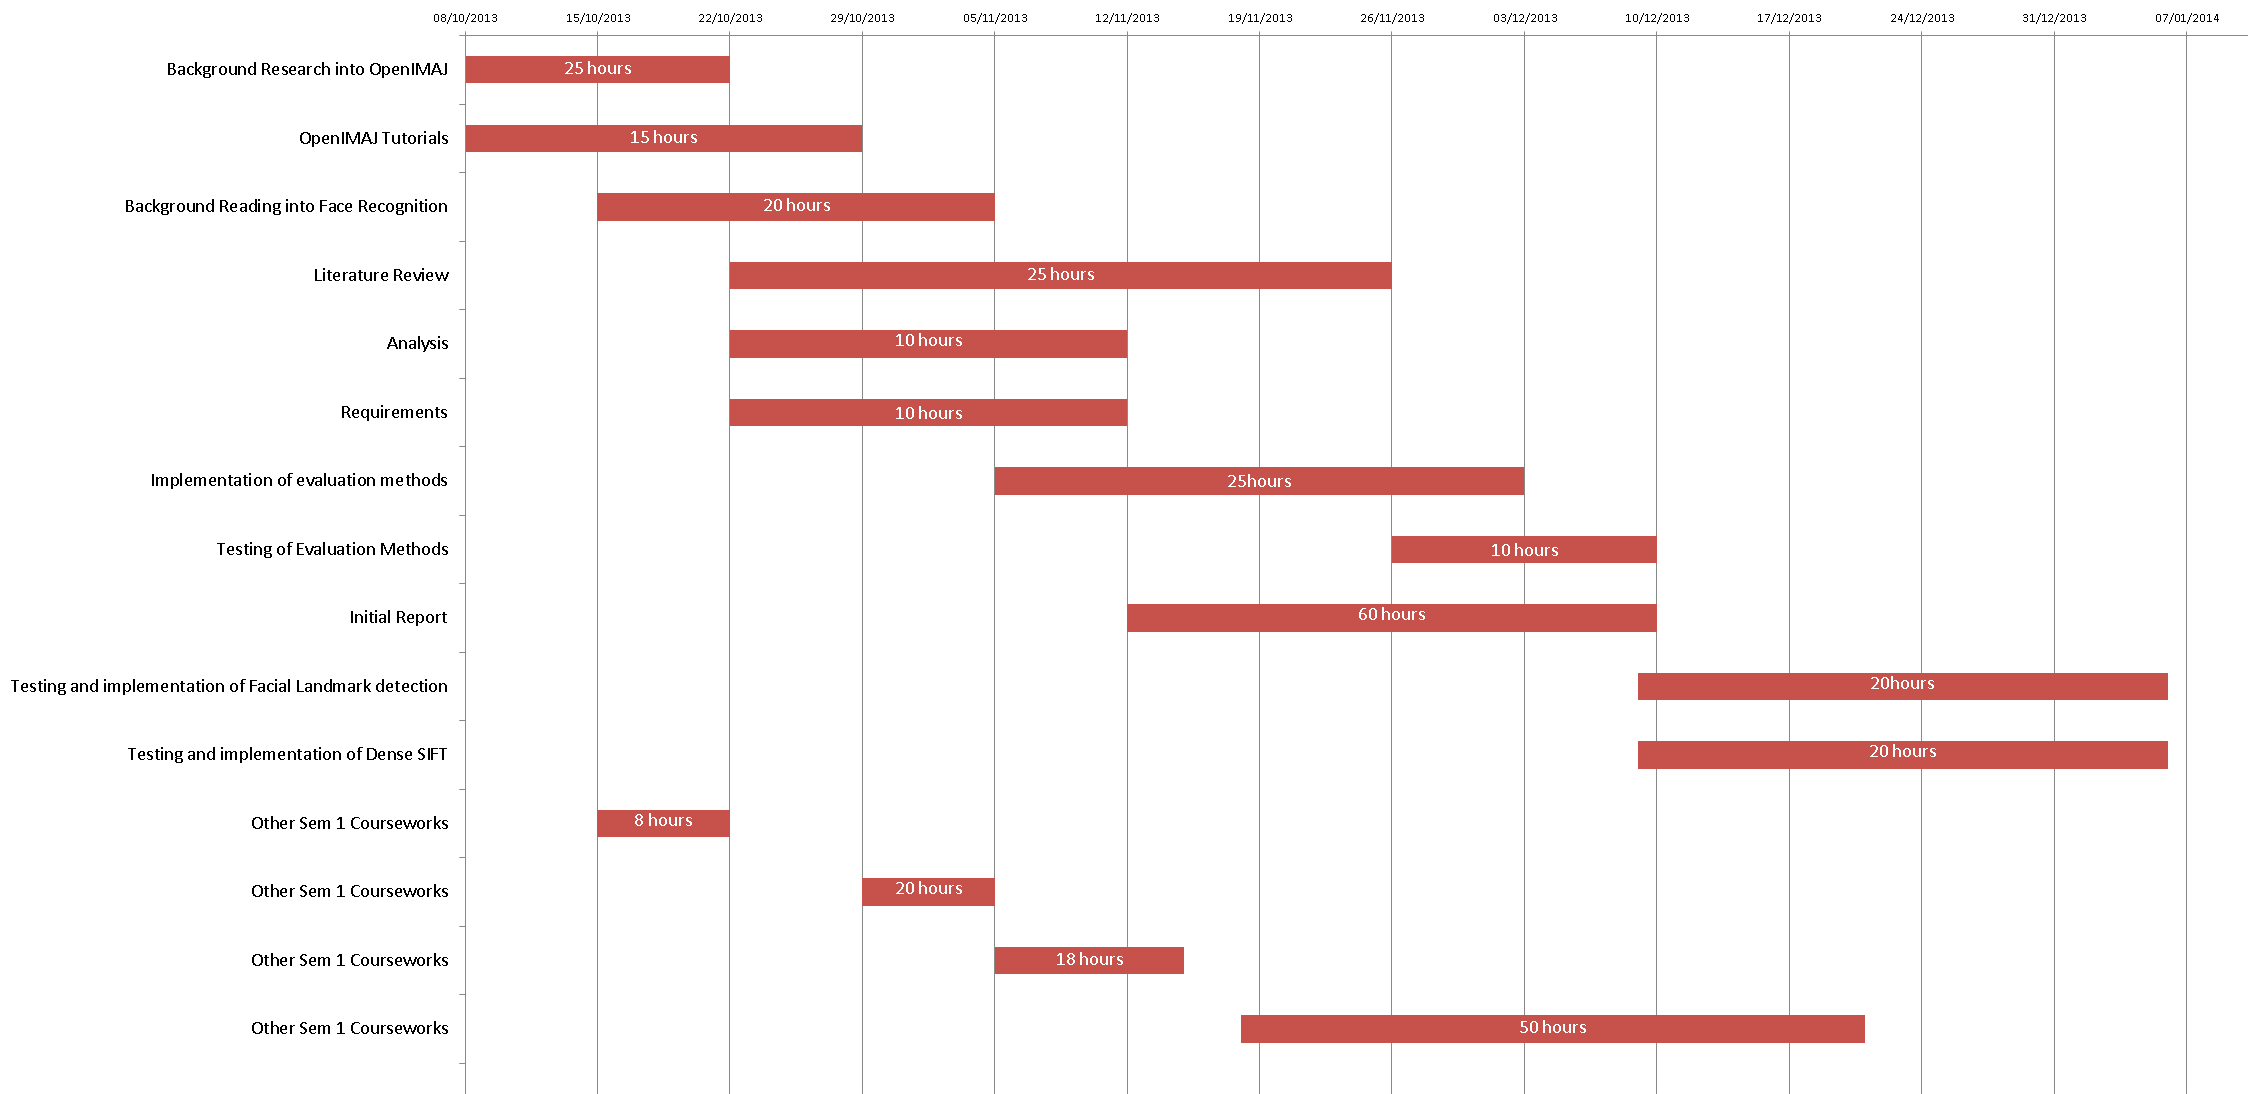
\includegraphics[scale=0.3, angle=90]{images/newganttprexmas.png}
\subsection{Updated Gantt Chart, work after Christmas}
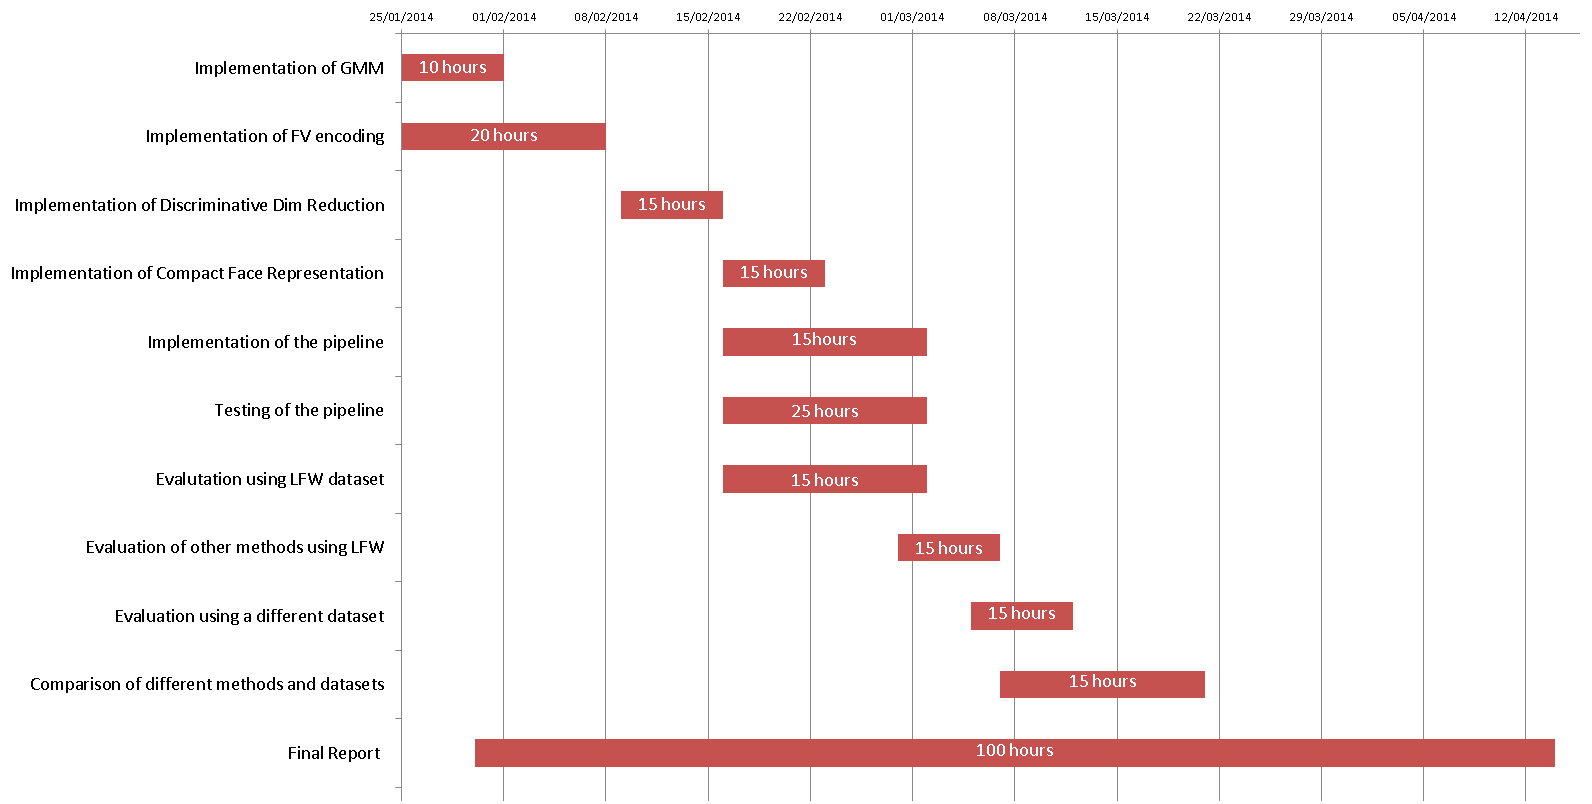
\includegraphics[scale=0.4, angle=90]{images/newganttpostxmas.png}

        \end{appendices}       
       
       
%%%%%%%%%%%%%%%%%%%%%%%%%
%      BIBLIOGRAPHY     %
%%%%%%%%%%%%%%%%%%%%%%%%%
        \newpage
 
        \bibliographystyle{abbrv}
\bibliography{final.bib}

\end{document}